\chapter{Related work}

In the introduction, we presented the programming language C\# and its possible improvement of type inference. 
This chapter continues by describing relevant sections of the C\# language and its type inference algorithm to understand the possible barriers to implement improved type inference. 
As a primary source of inspiration for the improvement, we will explore Hindley-Milner type inference in more detail and describe its modification in Rust and C\# programming languages. 
For the third goal of this thesis, we will mention relevant C\# language issues presented on the GitHub repository, which we use later to prioritize the improvement features to make it more likely to be accepted by \ac{LDM}. 

\section{C\# programming language}

\info{Explain purpose of this section}
Although C\# language features complement each other, we try to extract only relevant components for type inference in this section. 
We describe the type system, including C\# generics and their possibilities. 
Then, we mention unrelated language constructs that influence the type inference, and we have to count on them in proposing improved type inference. 
At the end of this section, we list types of type inference in C\# and describe them in necessary detail for the following chapters.

\subsection{Type system}

\info{Value/reference types}
\info{Inheritance}
As we mentioned in the introduction, each variable and expression returning a value has to have a type in the C\# type system \cite{online:cSharpTypeSystem} called the \ac{CTS}.
Its fundamental characteristic is type inheritance, where every type directly or indirectly inherits a base type \texttt{System.Object}, as you can see in the picture \ref{img04:typeSys}.
This chain of inheritance forms a tree, meaning that it is prohibited to inherit more than one type.
Types are divided into value and reference types.
Value types consist of built-in numeric types, structures (\texttt{struct}), and enumeration (\texttt{enum}).
Compared to classes (\texttt{class}) and records (\texttt{record}) belonging to reference types, value types can't be inherited by other types.
The last relevant member of reference types is interface (\texttt{interface}), which can extend multiple interfaces and be implemented by \texttt{class}, \texttt{record}, or \texttt{struct}.
\par
\begin{figure}[b!]
\centering
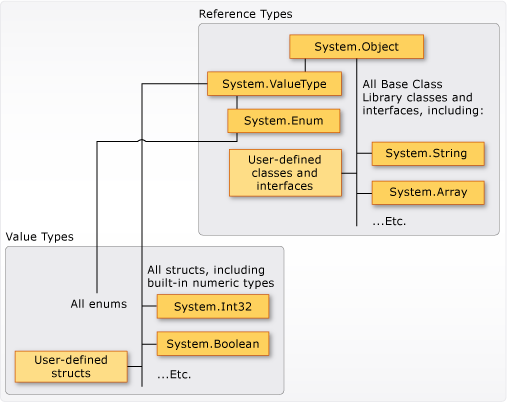
\includegraphics[width=140mm, height=100mm]{../img/value-reference-types-common-type-system.png}
\caption{The C\# type system \cite{online:cSharpTypeSystem}.}
\label{img04:typeSys}
\end{figure}
\par
\info{Nullability analysis}
C\# type inference infers, besides a type, its nullability, determining if it is possible to assign \texttt{null} value to that type.
C\# implicitly allows to assign \texttt{null} values to reference types indicating invalid value.
Since C\# 2.0 \cite{online:csHist}, it allows to assign \texttt{null} values to nullable value types, which are generic wrappers around value types.
Because assigning \texttt{null} value is referred to as a billion-dollar mistake, C\# 8.0 introduces optional settings prohibiting it and created nullable reference types explicitly allowing \texttt{null} assignment as a way of interaction with legacy code not using the feature.
\par
\info{Generic types and methods}
An essential part of the type system is C\# Generics, allowing parametrization of types and methods by other types. 
An example of a generic class is \texttt{System.Collections.Generic.List<T>} representing resizeable mutable array where  \texttt{T} represents arbitrary data type, which we want to have a collection of. 
Providing a type argument for  \texttt{T}, we create a new type where the type argument replaces the usages of  \texttt{T}.
\par
\info{Generic constraints}
Because a type parameter can be arbitrary, C\# treats it as a \texttt{System.Object}, which is insufficient in cases where the type parameter should provide special behaviour distinct from \texttt{System.Object}.
This requirement is achieved by type constraints, which restrict a set of types that can be passed to the parameter.
Several types of restrictions can be applied to type parameters in order to enable more actions on values of the restricted type parameters.
We can see examples of type constraints in the following code \ref{img05:typeConst}, where we use implementation restriction forcing the \texttt{T} to implement an interface providing API for comparing values with the same type.
The second restriction forces the type argument to have a default constructor.
Another restriction concerns an obligation that the type will be a value type or the type has to be non-nullable.
\par
\begin{figure}
\begin{lstlisting}[style=csharp]
class MyList<T> : where T : IComparable<T>, new()
{  
	private T[] myBuffer;
	
	int CompareOnIndicies(int idx1, int idx2) {
		return myBuffer[idx1].CompareTo(myBufffer[idx2])	
	}
}
\end{lstlisting}
\caption{C\# type constraints.}
\label{img05:typeConst}
\end{figure}
\par
\info{Variance and contra-variance}
The last feature of generics influencing type inference is the concept of type variance.
Initially, type parameters are invariant, meaning an obligation to assign a generic type to another generic type having the same types of type parameters.
Generic interfaces introduce additional modifiers (\texttt{in}, and \texttt{out}) of type parameters, which allow to assign a type with the more specialized type argument to a type with the less specialized type argument or vice-versa respectively.
\par
\info{Overloading}
We end this subsection by presenting method overloading. 
C\# allows the definition of multiple methods with the same and count of type arguments having different parameters. 
We will see in the following chapters why this feature is one of the barriers to implement strong and efficient type inference.

\subsection{Relevant constructs}

For this and the following section, we use the code example \ref{img55:typeConst} to better demonstrate the constructs and type inference.
\par
\info{Dynamic}
C\# type inference mostly happens at compile time, with one exception. 
We previously mentioned that C\# requires knowing the types of all variables and expressions during compilation. 
It turned out that the possibility of expressing type, which is unknown at compile time, became crucial for interoperability with other dynamic typed languages. 
To make the interoperability easier, C\# introduced a dynamic keyword that can be used as an ordinary type, which causes late binding of all expressions containing the dynamic value.
We can see an usage of the \texttt{dynamic} keyword on line 6 in the figure \ref{img55:typeConst} where we can notice the late binding on line 7 which doesn't cause a compile time error even the referring value doesn't define any method with the name \texttt{Foo}.
Internally, the type is \texttt{System.Object}, however, the compiler skips its binding and postpones it to the runtime.
Although the mentioned error on line 7 occurs at runtime, the compiler still attempts to check certain expressions containing dynamic values to reveal possible errors at compile time as we can see on line 8 where an error regarding of passing \texttt{System.String} to \texttt{System.Int} occurs during compilation.
\par
\info{Implicit typed lambdas}
The next language construct influencing type inference is an anonymous function, also known as Lambda, which, instead of declaring a dedicated method with a signature and a body, allows to specify only the body with untyped parameters on places where a function delegate is required.
We can see an example of Lambda expression on line 4 in the figure \ref{img55:typeConst} where we pass it as the fourth argument. 
Type inference infers its signature based on the surrounding context.
\par
\info{Object creation expression and initializers}
The last language feature which will take part in the improved type inference are initializers used as a shortcut during an object instantiation.
The most simple one is an object initializer that allows to assign values to the object's fields in a pleasant way instead of assigning them separately after the initialization.
The second type of initializers regard arrays and collections.
Array initializers are used to create fixed arrays with predefined content as we can see on the first line of our example \ref{img55:typeConst} where we create an array of \texttt{System.Object} with two items.
Under the hood, each of the items in the initializer is assigned to the corresponding index of the array after the array creation.
Collection initializers are similar to an array initializer defined on collections which are determined by implementing \texttt{ICollection<T>} interface.
One of the interface's declaring methods is \texttt{void Add<T>(T)} with adding semantic.
Each type implementing this interface is allowed to use an initializer list in the same manner as an array initializer.
It's just a sugar code hiding to call the `Add` method for each item in the initializer list.
The last type of initializer uses indexer to store referred values on predefined positions.
\par
\begin{figure}
\begin{lstlisting}[style=csharpN]
var myArray = new [] {new object(), "string"};
List<int> myList = new();

Helper.Method2((long)1, (int)1, myList, (p1) => p1 + 1);

dynamic dynamicValue = "string";
dynamicValue.Foo();
Helper.Method1("string", myArray, dynamicValue);

class Helper {
 static void Method1<T>(int p1, IList<T> p3) {...}
 static void
 Method2<T1, T2, T3>(T1 p1, T1 p2, IList<T2> p3, Func<T2, T3> p4)
 {...}
}
\end{lstlisting}
\caption{C\# code example.}
\label{img55:typeConst}
\end{figure}

\subsection{Type inference}

\info{Introduce kinds of type inferences}
\info{Method type inference}
C\# type inference occurs in many contexts. 
However, we mention only these related to our improvement described in the following sections. 
One of the most simple occurrences regards the \texttt{var} keyword, used in the variable declaration, as seen on the first line in code \ref{img55:typeConst}. It lets the compiler decide the type of variable based on the type of initializing value, which implies that we can’t use the keyword in declarations without initializing the value.
\par
The most interesting and complex context is the method type inference used during generic method call binding when type arguments are not given. 
We can see a situation when the method type inference deduces \texttt{System.String}, \texttt{System.Int32} and \texttt{System.Int32} as type arguments of the \texttt{MyMethod} method on line 4 in our code example \ref{img55:typeConst}. 
We can notice several tasks that the type inference has to be capable of.
Regarding the \texttt{T1} type parameter, the inference has to find a common type between the first and the second type parameters. 
Regarding the \texttt{T2} type parameter, the type inference has to go into type arguments of the generic type of parameter and the argument, check if the types are compatible, and then match the type parameter against the type argument of the third parameter. 
The most challenging is Lamdas, whose return type has to be inferred after all lambda argument types are inferred.
\par
As we can see, the method type inference is a complex process containing many steps.
Since one of our improvements is adjusting the algorithm, we present its complete description.
The algorithm is divided into four sections to explain its functionality better.
Before we show schema, we have to present definitions that are used by the algorithm referred in \cite{online:csTypeInference}.
\par
\begin{defn}[Fixed type variables, bounds]
We call inferred type parameters \emph{type variables} which are at the beginning of the algorithm unknown, \emph{unfixed}. 
During the algorithm, they start to be restricted by sets of type \emph{bounds}.
The type variable becomes \emph{fixed} when the its actual type is determined using its \emph{bounds}.
\end{defn}
\begin{defn}[Method group]
A \emph{method group} is a set of overloaded methods resulting from a member lookup.
\end{defn}
\begin{defn}[Input/Output types]
If \texttt{E} is a method group or anonymous function and \texttt{T} is a delegate or expression tree type, then return type of \texttt{T} is an \emph{output type} of \texttt{E}.
If \texttt{E} is a method group or implicitly typed anonymous function, then all the parameter types of \texttt{T} are \emph{input types} of \texttt{E}. 
\end{defn}
\par
\begin{defn}[Dependence]
An unfixed type variable \texttt{$X_i$} \emph{depends directly on} an unfixed type variable \texttt{$X_e$} if for some argument \texttt{E} \texttt{$X_e$} occurs in an input type of \texttt{E} and \texttt{$X_i$} occurs in an output type of \texttt{E}.
\texttt{$X_i$} \emph{depends on} \texttt{$X_e$} is the transitive but not reflexive closure of \emph{depends directly on}.
\end{defn}
\par
\info{Algorithm description}
The method type inference process starts with receiving arguments of a method call and the method's signature, which type parameters have to be deduced, as we can see in the first schema \ref{alg01:methodTypeInference1}.
The algorithm has two phases where the first phase initializes initial bounds' sets of type variables(inferred type arguments), and the second phase repeats until all type variables are fixed or fails if there is insufficient information to deduce it.
Each type variable has three types of bounds. 
The exact bound consists of types, which have to be identical to the type variable, meaning that they can be converted to each other.
The lower bound contains types that have to be convertible to the type variable, and the upper bound is opposite to it. 
\par
\begin{algorithm}
\SetKwFunction{FirstPhase}{FirstPhase}
\SetKwFunction{SecondPhase}{SecondPhase}
\SetKwFunction{InferExplicitParameterType}{InferExplicitParameterType}
\SetKwFunction{InferExact}{InferExact}
\SetKwFunction{InferLowerBound}{InferLowerBound}
\SetKwFunction{isValueParameter}{isValParam}
\SetKwFunction{isReferenceParameter}{isRefParam}
\SetKwFunction{isInputParameter}{isInParam}
\SetKwFunction{isInputArgument}{isInArg}
\SetKwFunction{isOutputParameter}{isOutParam}
\SetKwFunction{Fix}{Fix}
\SetKwFunction{Failed}{Failed}
\SetKwFunction{Return}{Return}
\SetKwFunction{inputTypes}{inTypes}
\SetKwFunction{outputTypes}{outTypes}
\SetKwFunction{GoTo}{GoTo}
\SetKwFunction{InferOutputType}{InferOutputType}
\SetKwProg{Fn}{fn}{:}{}

\KwIn{a method call \texttt{M($\mathtt{E_1, ..., E_x}$)} and its signature \texttt{$\mathtt{T_e}$ M<$\mathtt{X_1, ..., X_n}$>($\mathtt{T_1 p_1, ..., T_x p_x}$)}}
\KwOut{$X_1, ..., X_n$}
$B_{lower}, B_{upper}, B_{exact}, F \gets [\ ]$\;
\FirstPhase{}\;
\SecondPhase{}\;
\Fn{\FirstPhase{}}{
	\ForEach{$E_i$}{
		\If{$E_i$ $\in$ AnonymousFuncs}{
			\InferExplicitParameterType{$E_i, T_i$}
		}
		\ElseIf{$E_i$ has a type $U$}{
			\Switch(\tcc*[h]{At most one case is executed}){$U$}{
				\lCase{\isValueParameter{$p_i$}}{\InferLowerBound($U, T_i$)}
				\Case{\isReferenceParameter{$p_i$} $\vee$ \isOutputParameter{$p_i$}}{\InferExact{$U, T_i$}}
				\Case{\isInputParameter{$p_i$} $\wedge$ \isInputArgument{$E_i$}}{\InferExact{$U, T_i$}}
				\lCase{\isInputParameter{$p_i$}}{\InferLowerBound{$U, T_i$}}
			}
		}
	}
}
\Fn{\SecondPhase{}}{
	$X_{indep} \gets \forall X_i : F[i] = null \wedge \nexists X_e : dependsOn(X_i, X_e)$\;
	$X_{dep} \gets \forall X_i\ :\ F[i] = null\ \wedge (\exists X_e : dependsOn(X_e, X_i) \vee B_{lower}[i] \cup B_{exact}[i] \cup B_{upper}[i] \neq empty)$\;
	\Switch{$X_{indep}$, $X_{dep}$}{
		\Case{$X_{indep}$ $\neq$ empty}{
			\lForEach{$X_s$ $\in$ $X_{indep}$}{\Fix{$X_s$}}		
		}
		\Case{$X_{indep}$ = empty $\wedge$ $X_{dependent}$ $\neq$ empty}{
			\lForEach{$X_s$ $\in$ $X_{indep}$}{\Fix{$X_s$}}				
		}
		\Case{$X_{indep}$ $\cup$ $X_{dep}$ = empty}{
		\lIf{$\exists X_k$ : F[k] = null}{\Failed{}}
		\lElse{\Return{F[0], ..., F[n]}}
		}
		\Other{
			\lForEach{$E_i$ : $\exists$ $X_e$ : F[e] = null $\wedge$ $X_e$ $\in$  \outputTypes{$T_i$} $\wedge$ $\nexists$ $X_k$ : F[k] = null $\wedge$ $X_k$ $\in$ \inputTypes{$T_i$}}{
				\InferOutputType{$E_i, T_i$}			
			}	
			\GoTo{\normalfont\texttt{16}}	
		}
	}
}
\caption{Phases of Method Type Inference}
\label{alg01:methodTypeInference1}
\end{algorithm}
\par
\info{The first phase description}
The first phase iterates over provided arguments and chooses the right set where to add the type of the argument by calling helper functions based on several conditions.
We suppose the reader has knowledge of C\# language, so we quickly mention used functions contained in the conditions for clarifying meant constructs of parameters and arguments.
\texttt{isValParam()} and \texttt{isRefParam()} functions determine if the parameter is passed by value or by reference.
There are also \texttt{isInParam()}, \texttt{isOutParam()}, \texttt{isInArg()} referring to the use of \texttt{in} and \texttt{out} keywords in parameter declarations and \texttt{in} keyword in the argument position.
\info{The second phase description}
The second phase happens iteratively, respecting \textit{depends on} relation.
Each iteration has two goals.
The first one is the fixation of at least one type variable.
If there is no type variable to fix because either all type variables are fixed or there are no other type bounds which could be used for type variable deduction, the phases and algorithm ends.
The sets \texttt{$X_{indep}$} and \texttt{$X_{dep}$} refer to type variables, which can be fixed in the current iteration.
Line 24 contains a case ending the algorithm when all type variables are fixed, or there is no way to infer the next ones.
The second goal checks for output types, dependent on input types where the last unfixed types were fixed in this iteration, and infers them.
We can see respecting the order of inferring the return type of anonymous functions at line 29, where the return type of lambdas is inferred if all type variables contained in the parameter list are fixed.
\par
\info{Describe infer output type}
Algorithm \ref{alg02:methodTypeInference2} contains definitions of three inferences used in the first and second phases.
\texttt{InferOutputType()} infers return types of parameter types, which are delegates or expression trees.
We can notice two situations where the first one takes care of arguments, which are Lambdas, and the second deals with method groups with possible type arguments. 
We can see two undefined methods used to achieve the inference above.
\texttt{InferReturnType()} utilizes already known types of lambdas argument to infer its return type.
\texttt{OverloadResolution} tries resolving a method group to one method in order to infer the return type of that method.
\par
\info{Describe infer explicit parameter type}
\texttt{ExplicitParamterType()} method is used when an argument is explicitly typed anonymous function where the given parameter types are used to get information about type variables contained in a parameter of delegate or expression tree type.
\par
\info{Describe infer exact}
\texttt{InferExact()} is one of the three inferences which adds new bounds to type variables' bound sets.
Basically, it finds arguments' types with corresponding parameter types and adds these types to the bounds when they match type variables as we can see at line 16.
\par
\begin{algorithm}
\SetKwFunction{OverloadResolution}{OverloadResolution}
\SetKwFunction{InferOutputType}{InferOutputType}
\SetKwFunction{InferExplicitParameterType}{InferExplicitParameterType}
\SetKwFunction{InferReturnType}{InferReturnType}
\SetKwFunction{InferExact}{InferExact}
\SetKwFunction{InferLower}{InferLower}
\SetKwFunction{Add}{Add}
\SetKwProg{Fn}{fn}{:}{}

\Fn{\InferOutputType{E, T}}{
	\Switch{E}{
		\Case{E $\in$ AnonymousFuncs $\wedge$ T $\in$ DelegateTypes $\cup$ ExprTreeTypes}{
			\InferLower{\InferReturnType{E}, T.ReturnType}		
		}
		\Case{E $\in$ MethGroups $\wedge$ T $\in$ DelegateTypes $\cup$ ExprTreeTypes}{
			$T_{ret}, T_1,...T_n \gets T.ReturnType, T.ParamTypes$\; 
			$E_{resolved}$ $\gets$ \OverloadResolution{$E, T_1,...T_n$}\;
			\If{$\|E_{resolved}\|$ = 1}{
				\InferLower{$E_{resolved}[1].ReturnType, _{ret}$}			
			}
		}
		\lCase{E $\in$ Expressions $\wedge$ E has a type U}{
			\InferLower{U, T}
		}	
	}
}
\Fn{\InferExplicitParameterType{E, T}}{
	\If{E $\in$ ExplicitlyTypedAnonymousFuncs $\wedge$ T $\in$ DelegateTypes $\cup$ ExprTreeTypes $\wedge$ $\|E.ParamTypes\| = \|T.ParamTypes\|$}{
		\ForEach{$U_i, V_i$ : $U_i$ $\in$ E.ParamTypes $\wedge$ $V_i$ $\in$ T.ParamTypes}{
			\InferExact{$U_i, V_i$}		
		}	
	}
}
\Fn{\InferExact{U, V}}{
	\lIf{$\exists$ i : V = $X_i$ $\wedge$ F[i] = null }{
		$B_{exact}[i]$.\Add{U}	
	}
	\Switch{V}{
		\Case{V = $V_1$[...] $\wedge$ U = $U_1$[...] $\wedge$ V.Rank = U.Rank}{
			\InferExact{$U_1, V_1$}		
		}
		\lCase{V = \normalfont\texttt{$V_1$?} $\wedge$ U = $U_1$}{
			\InferExact{$V_1, U_1$}		
		}
		\Case{V = \normalfont\texttt{C<$V_1,...V_e$>} $\wedge$ U = \normalfont\texttt{C<$U_1,...U_e$>}}{
			\lForEach{$V_i, U_i$}{
				\InferExact{$V_i, U_i$}
			}		
		}
	}	
}
\caption{\textit{Output type inference}, \textit{Explicit parameter type inference}, \textit{Exact inference}}
\label{alg02:methodTypeInference2}
\end{algorithm}
\par
\info{Describe infer lower, upper}
Algorithm \ref{alg03:methodTypeInference3} shows remaining two inferences, adding types to lower and upper bounds.
We can see various conditions testing corresponding types between arguments and parameters. 
An interesting fact about adding new bounds is that there is no need to check possible contradictions, which are checked in type variable fixation. 
The second point that will be important for us in the following sections is the absence of unfixed type variables in bound sets, making the algorithm easier for implementation.
\par
\begin{algorithm}
\SetKwFunction{InferExact}{InferExact}
\SetKwFunction{InferLower}{InferLower}
\SetKwFunction{InferUpper}{InferUpper}
\SetKwFunction{isReferenceType}{isRefType}
\SetKwFunction{Add}{Add}
\SetKwFunction{IdenticalTo}{IdenticalTo}
\SetKwFunction{Inherits}{Inherits}
\SetKwFunction{Implements}{Implements}
\SetKwFunction{isCovariant}{isCovariant}
\SetKwFunction{isContravariant}{isContravariant}
\SetKwFunction{isInvariant}{isInvariant}
\SetKwProg{Fn}{fn}{:}{}


\Fn{\InferLower{U, V}}{
	\lIf{$\exists$ i : V = $X_i$ $\wedge$ F[i] = null }{
		$B_{lower}[i]$.\Add{U}	
	}
	\Switch{V, U}{
		\lCase{V = \normalfont\texttt{$V_1$?} $\wedge$ U = \normalfont\texttt{$U_1$?}}{
			\InferLower{$V_1, U_1$}		
		}
		\Case{V = $V_1$[...] $\wedge$ U = $U_1$[...] $\wedge$ V.Rank = U.Rank}{
			\lIf{\normalfont\texttt{!}\isReferenceType{$U_1$}}{
				\InferExact{$U_1$, $V_1$}		
			}
			\lElse{
				\InferLower($U_1$, $V_1$)			
			}
		}
		\Case{V $\in$ \{\normalfont\texttt{IEnumerable<$V_1$>}, \normalfont\texttt{ICollection<$V_1$>}, \normalfont\texttt{IReadOnlyCollection<$V_1$>}, \normalfont\texttt{IReadOnlyCollection<$V_1$>}, \normalfont\texttt{IList<$V_1$>}\} $\wedge$ U = $U_1$[ ]}{
			\lIf{\isReferenceType{$U_1$}}{
				\InferExact{$U_1$, $V_1$}		
			}
			\lElse{
				\InferLower($U_1$, $V_1$)			
			}
		}
		\Case{V = \normalfont\texttt{C<$V_1, ..., V_e$>} $\wedge$ $\exists!$ \normalfont\texttt{C<$U_1, ..., U_e$>} : \IdenticalTo{U, \normalfont\texttt{C<$U_1, ..., U_e$>}} $\vee$ \Inherits{U, \normalfont\texttt{C<$U_1, ..., U_e$>}} $\vee$ \Implements{U, \normalfont\texttt{C<$U_1, ..., U_e$>}}}{
			\Switch{${V_i}$}{
				\lCase{\isCovariant{${V_i}$}}{
					\InferLower{${U_i}$, ${V_i}$}
				}
				\lCase{\isContravariant{${V_i}$}}{
					\InferUpper{${U_i}$, ${V_i}$}
				}
				\lCase{\isInvariant{${V_i}$}}{
					\InferExact{${U_i}$, ${V_i}$}
				}			
			}
		}
	}
}
\Fn{\InferUpper{U, V}}{
	\lIf{$\exists$ i : V = $X_i$ $\wedge$ F[i] = null }{
		$B_{upper}[i]$.\Add{U}	
	}
	\Switch{V, U}{
		\Case{V = \normalfont\texttt{$V_1$?} $\wedge$ U = \normalfont\texttt{$U_1$?}}{
			\lIf{\normalfont\texttt{!}\isReferenceType{$U_1$}}{
				\InferExact{$U_1$, $V_1$}		
			}
			\lElse{
				\InferUpper($U_1$, $V_1$)			
			}
		}
		\Case{V = $V_1$[...] $\wedge$ U = $U_1$[...] $\wedge$ V.Rank = U.Rank}{
			\lIf{\normalfont\texttt{!}\isReferenceType{$U_1$}}{
				\InferExact{$U_1$, $V_1$}		
			}
			\lElse{
				\InferUpper($U_1$, $V_1$)			
			}
		}
		\Case{U $\in$ \{\normalfont\texttt{IEnumerable<$U_1$>}, \normalfont\texttt{ICollection<$U_1$>}, \normalfont\texttt{IReadOnlyCollection<$U_1$>}, \normalfont\texttt{IReadOnlyCollection<$U_1$>}, \normalfont\texttt{IList<$U_1$>}\} $\wedge$ V = $V_1$[ ]}{
			\lIf{\isReferenceType{$U_1$}}{
				\InferExact{$U_1$, $V_1$}		
			}
			\lElse{
				\InferLower($U_1$, $V_1$)			
			}
		}
		\Case{U = \normalfont\texttt{C<$U_1, ..., U_e$>} $\wedge$ $\exists!$ \normalfont\texttt{C<$V_1, ..., V_e$>} : \IdenticalTo{V, \normalfont\texttt{C<$V_1, ..., V_e$>}} $\vee$ \Inherits{V, \normalfont\texttt{C<$V_1, ..., V_e$>}} $\vee$ \Implements{V, \normalfont\texttt{C<$V_1, ..., V_e$>}}}{
			\Switch{${U_i}$}{
				\lCase{\isCovariant{${U_i}$}}{
					\InferUpper{${U_i}$, ${V_i}$}
				}
				\lCase{\isContravariant{${U_i}$}}{
					\InferLower{${U_i}$, ${V_i}$}
				}
				\lCase{\isInvariant{${U_i}$}}{
					\InferExact{${U_i}$, ${V_i}$}
				}			
			}
		}
	}
}
\caption{\textit{Upper-bound inference}, \textit{Lower-bound inference}}
\label{alg03:methodTypeInference3}
\end{algorithm}
\par
\info{Fix}
The last part of this algorithm is type variable fixation, shown in algorithm  \ref{alg04:methodTypeInference4}.
At the beginning, a set of candidates for the type variable is constructed by collecting all its bounds. 
Then, we go through each bounds and remove the candidates which do not satisfy the bound’s restriction. 
If there is more than one candidate left, we try to find a unique type that is identical to all left candidates.
The fixation is successful if the candidate is found.
The type variable is fixed to that type.
\par
\begin{algorithm}
\SetKwFunction{IdenticalTo}{IdenticalTo}
\SetKwFunction{hasImplicitConversion}{hasImplicitConversion}
\SetKwFunction{Failed}{Failed}
\SetKwFunction{Fix}{Fix}
\SetKwProg{Fn}{fn}{:}{}

\Fn{\Fix{$X_i$}}{
	$U_{candidates} \gets B_{upper}[i] \cup B_{exact}[i] \cup B_{lower}[i]$\;
	\ForEach{U ${\in}$ $B_{exact}[i]$}{
		$U_{candidates}$ -= \{$U_r$ : $U_r$ $\in$ $U_{candidates}$ $\wedge$ \normalfont\texttt{!}\IdenticalTo{$U_r$, U}\}
	}
	\ForEach{U ${\in}$ $B_{lower}[i]$}{
		$U_{candidates}$ -= \{$U_r$ : $U_r$ $\in$ $U_{candidates}$ $\wedge$ \normalfont\texttt{!}\hasImplicitConversion{U, $U_r$}\}
	}
	\ForEach{U ${\in}$ $B_{upper}[i]$}{
		$U_{candidates}$ -= \{$U_r$ : $U_r$ $\in$ $U_{candidates}$ $\wedge$ \normalfont\texttt{!}\hasImplicitConversion{$U_r$, U}\}
	}
	\lIf{$\exists!$ V : V $\in$ $U_{candidates}$ $\wedge$ $\forall$ $U_e$ $\in$ $U_{candidates}$ : \hasImplicitConversion{$U_e, V$}}{
		F[i] = V
	}
	\lElse{
		Failed()
	}
}
\caption{Fixing of type variables}
\label{alg04:methodTypeInference4}
\end{algorithm}
\info{Array type inference}
The third type inference happens in array initializers when the type of the array should be deduced from the initializer list.
We can see an example of a situation when the type inference is used for determining \texttt{myArray} type on the first line in our code example \ref{img55:typeConst}.
The most specialized common type is just adjusted already mentioned type inference algorithm where there is just one type parameter, and all initializer items are lower bounds of that type variable.
\par
\info{Target-typed inference}
The last kind of type inference, which we mention, regards inference based on target type.
An example of these situations can be seen on the second line of our example \ref{img55:typeConst} where we use target-typed \texttt{new()} operator, allowing us to skip creating type, which is provided by the target type, variable type, in this case.

\section{Roslyn}

\info{Intro}
The implementation of C\# type inference can be found in the Roslyn compiler, as open-source C\# and VisualBasic compiler developed at the GitHub repository. 
In this section, we present Roslyn’s architecture to better understand the context and restrictions that we must consider to plug the improved type inference into the compiler.
\par
\begin{figure}
\centering
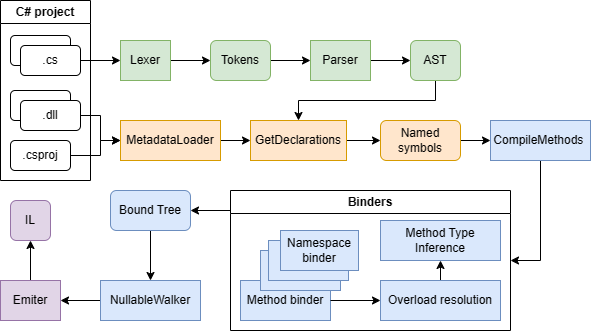
\includegraphics[width=120mm, height=70mm]{../img/Roslyn_Arch.png}
\caption{Roslyn architecture}
\label{img56:roslynPip}
\end{figure}
\par
\info{Overview of compilation pipeline, the first phase}
The compilation pipeline, described in \cite{online:roslynArchitecture}, starts with loading the \texttt{.csproj} file with related C\# sources (\texttt{.cs}) and referenced libraries (\texttt{.dll}), as we can see in Figure \ref{img56:roslynPip}.
C\# sources are passed to the lexer, creating tokens used by the parser forming \ac{AST}.
Constructing \ac{AST} is the first phase (green color boxes of Figure \ref{img56:roslynPip}) of the compiler checking syntax of C\# sources.
\par
\info{Describe the second phase}
The second phase, marked by orange, forms \emph{Named symbols} exposed by public API representing defined namespaces, classes, methods, etc., in the C\# project. 
The declarations are received from C\# sources by traversing AST and seeking for the particular syntax. Stored in \texttt{.dll} format, Libraries are parsed by \texttt{MetadataLoader}, creating the same Named symbols as those received from C\# sources.
\par
\info{Describe the third phase}
The third phase, also called the binding phase, matches identifiers in the code with received Named symbols from the previous phase. 
Because the processing of a method body is not dependent on other method bodies since the code only uses already known declarations, Roslyn makes this phase concurrent. 
The result of the phase is a \emph{Bound tree} where all identifiers refer to the Named symbols. 
A method binding itself is a complicated procedure consisting of many subtasks such as \emph{Overload resolution} or mentioned Method type inference, which algorithm we described in detail in the previous section.
\par
\info{Binder}
The binding is divided into a chain of binders, taking care of smaller code scopes. 
One purpose of the binders is the ability to resolve an identifier to the Named symbol if the referred symbol lies in their scope. 
If they can’t find the symbol, they ask the preceding binder. 
This process is called \emph{LookUp}, determining which Named symbols are accessible in the current position. 
Examples of binders are \texttt{NamespaceBinder} resolving defined top-level entities in the namespace scope, \texttt{ClassBinder} resolving defined class members, or \texttt{MethodBinder} binding method bodies. 
The last mentioned binder sequentially iterates body statements and matches identifiers with their declarations. 
Statement and expression binding are important steps that are related to type inference. 
The first observation is that statement binding doesn’t involve binding of the following statements, which can be referred to as backward binding. 
The consequence is that C\# is not able to infer types in the backward direction. 
An example can be the usage of the \texttt{var} keyword in variable declarations, which has to be used always with initializing value. 
If C\# would allow backward binding, we could initialize the variable later in one of the following statements.
\par
\info{OverloadResolution, MethodTypeInferrer}
The preceding step before Method type inference is Overload resolution, part of \texttt{MethodCallExpression} or \texttt{ObjectCreationExpression} binding. 
As we mentioned previously, method overloading allows to define multiple methods with the same name differing in parameters. 
So, when deciding which method should be called, we have to resolve the right version of the method by following language rules for method resolution. 
This step involves binding the method call arguments first and then deciding which parameter list of the method group fits the argument list the best. 
If the method group is generic and the expression doesn’t specify any type arguments, Method type inference is invoked to determine the type arguments of the method before the selection of the best candidate for the call.
\par
\info{NullableWalker}
Method type inference can occur for the second time if we turn on the nullability analysis mentioned previously. 
Nullability analysis is a kind of Flow analysis that uses a Bound tree to check and rewrite already created bound nodes according to nullability. 
Because overloading and method type inference are nullable-sensitive, the whole binding process is repeated, respecting the nullability and reusing results from the previous binding. 
The required changes are stored during the analysis, and the Bound tree is rewritten by the changes at the end of the analysis.

\section{Hindley-Millner type inference}

\info{Intro}
C\# method type inference is a restricted Hindley-Millner type inference in order to work in its C\# type system.
Since type inferences in other languages like Rust or Haskell are based on the same principle, we present a high-level overview of Hindley-Millner type inference and its type system to reason about possible extensions of current C\# type inference.
\info{Hindley-Millner type system}
Hindley-Millner type system \cite{online:wikiHM} is a type system for Lambda calculus capable of generic functions and types.
We start with describing a set of expressions, which will be a target of type inference described in the video series \cite{online:HMVideos}.
Expression is either a variable (\ref{expr01}), a function application (\ref{expr02}), a lambda function (\ref{expr03}), or a \textit{let-in} clause (\ref{expr04}).
\par
\begin{align}
e =&\ x\label{expr01}\\
|&\ e_1 e_2\label{expr02}\\
|&\ \lambda x \rightarrow e\label{expr03}\\
|&\ \text{\textbf{let}}\ x = e_1\ \text{\textbf{in}}\ e_2\label{expr04} 
\end{align}
\par
The above-mentioned expressions have one of two different types.
\textit{Mono} type is presented either as a type variable(\ref{type01}) or as a function application(\ref{type02}) where \textit{C} is an item from an arbitrary set of functions containing at least \texttt{$\rightarrow$} symbol taking two type parameters which represents a lambda function type.
The second group is \textit{Poly} types, which assemble from a type possible preceding $\forall$ operator \ref{type04}, bounding its type variables.
\par
\begin{align}
mono\ \tau =&\ \alpha\label{type01}\\
|&\ C\ \tau_1,...,\tau_n\label{type02}\\
poly\ \sigma =&\ \tau\label{type03}\\
|&\ \forall \alpha\ .\ \sigma\label{type04}
\end{align}
To be able to reason about more complex type expressions, a context(\texttt{$\Gamma$}) gives us assumptions of a current scope where we evaluate the type of expression.
It contains pairs of expressions and their types from which we can make typing judgments (using \texttt{$\vdash$} operator). 
\par
\info{Set of rules}
The H-M deduction system gives us the following inference rules, allowing us to deduce the type of an expression based on the assumption given in the context. 
The syntax of the rule corresponds with what we can judge (the right side of $\vdash$) from the left side of $\vdash$ below the line based on assumptions given above the line.
The rules can be divided into two kinds.
The first four rules give us a manual on what types we can expect by applying the mentioned expressions of Lambda calculus. 
The two last rules allow us to specify Poly types to Mono types and vice-versa.
\begin{align*}
\frac{x : \sigma \in \Gamma}{\Gamma \vdash x : \sigma}&[Var]\\
\frac{\Gamma \vdash e_0 : \tau_a \rightarrow \tau_b\ \ \ \Gamma \vdash e_1 : \tau_a}{\Gamma \vdash e_0 e_1 : \tau_b}&[App]\\
\frac{\Gamma, x : \tau_a \vdash e : \tau_b}{\Gamma \vdash \lambda x \rightarrow e : \tau_a \rightarrow \tau_b}&[Abs]\\
\frac{\Gamma \rightarrow e_0 : \sigma \ \ \ \Gamma , x : \sigma \vdash e_1 : \tau}{\Gamma \vdash\ \text{\textbf{let}}\ x = e_0\ \text{\textbf{in}}\ e_1 : \tau}&[Let]\\
\frac{\Gamma \vdash e : \sigma_a \ \ \ \sigma_a \sqsubseteq \sigma_b}{\Gamma \vdash e : \sigma_b}&[Inst]\\
\frac{\Gamma \vdash e : \sigma \ \ \ \alpha \notin Free(\Gamma)}{\Gamma \vdash e : \forall \alpha\ .\ \sigma}&[Gen]\\
\end{align*}
\par
\info{Describe type inference}
With the definitions given above, we can start to talk about H-M type inference, which is able to find the type of every expression of a completely untyped program.
There exist several algorithms for inferring most general type of the expression.
We show the W algorithm in schema \ref{alg05:w} since it is closely related to C\# and Rust type inference.
Inputs are the context $\Gamma$ and an expression which type we want to infer.
The process consists of systematic traversing the expression from bottom to top and deducing the type of sub-expressions following the mentioned rules.
The algorithm uses the \texttt{Instantiate} method to replace quantified type variables in the expression with new type variables, the \texttt{Generelize} method to replace free type variables in the expression with quantified type variables, and the \texttt{Unify} method, also known as \textit{Unification} in Logic.
Unification is an algorithm finding a substitution whose application on the unifying types makes them identical. 
Outputs of this algorithm are the inferred type with a substitution used for the algorithm's internal state. 
\par
\begin{algorithm}
\SetKwProg{Fn}{fn}{:}{}
\SetKwFunction{Infer}{Infer}
\SetKwFunction{Instantiate}{Instantiate}
\SetKwFunction{Generelize}{Generelize}
\SetKwFunction{NewVar}{NewVar}
\SetKwFunction{Unify}{Unify}
\SetKw{Ret}{return}

\Fn{\Infer{$\Gamma$, expr}}{
	\Switch{expr}{
		\Case{expr is \normalfont{x}}{
			\Ret (\{\}, \Instantiate{expr})		
		}
		\Case{expr is \normalfont{$\lambda$x$\rightarrow$e}}{
			$\beta$ $\gets$ \NewVar{}\;
			($S_1$, $\tau_1$) $\gets$ \Infer{$\Gamma$ + x : $\beta$, e}\;			
			\Ret ($S_1$, $S_1 \beta$ $\rightarrow$ $\tau_1$)
		}
		\Case{expr is \normalfont{$e_1e_2$}}{
			($S_1$,$\tau_1$) $\gets$ \Infer{$\Gamma$, $e_1$}\;
			($S_2$,$\tau_2$) $\gets$ \Infer{$S_1 \Gamma$, $e_2$}\;
			$\beta$ $\gets$ \NewVar{}\;
			$S_3$ $\gets$ \Unify{$S_2 \tau_1$ ,$\tau_2 \rightarrow \beta$}\;
			\Ret ($S_3 S_2 S_1$,$S_3 \beta$)		
		}
		\Case{expr is \normalfont{let x = $e_1$ in $e_2$}}{
			($S_1$, $\tau_1$) $\gets$ \Infer{$\Gamma$, $e_1$}\;
			($S_2$, $\tau_2$) $\gets$ \Infer{$\Gamma$ + x : \Generelize{$S_1 \Gamma$, $\tau_1$}, $e_2$}\;
			\Ret{$S_2 S_1$,$\tau_2$}
		}
	}
}
\caption{\textit{W} algorithm}
\label{alg05:w}
\end{algorithm}
\par
\info{Mention relation to Method type inference}
Relations between this algorithm and C\#, Rust type inference will be discussed in detail later, although we can notice that the unification part of this algorithm is the same as Method type inference mentioned in the C\# section where the substitution represents inferred type arguments of the method which parameters were unified with matching arguments.
\par
\info{Restriction and possible extensions - subtyping, overloading}
H-M type system, as we presented, doesn't allow subtyping known from Rust or overloading known from C\#.  
\par
A basic principle of extending H-M type inference by subtyping is described in Parreaux's work \cite{paper:Parreaux}, where instead of accumulating type equivalent constraints, we accumulate and propagate subtyping constraints.
These subtyping constraints assemble a set of types, which have to be inherited by the constrained type variable, or the variable has to inherit them.
\par
\info{Restriction and possible extensions - overloading}
Extending H-M type inference by supporting overloading mentions Andreas Stadelmeier and Martin Plumicke's work \cite{paper:Overloading}.
An important thought behind this paper is to accumulate two types of type variable constraint sets.
Constraints observed from a method call are added into one \textit{AND-set}.
When the method call has multiple overloads, the AND-sets are added to the \textit{OR-set}.
After accumulating these sets, all combinations of items in OR-sets are generated and solved by type inference.
As we can see, for each method overload participating in type inference, we have to make an alternative type inference containing constraints obtained only from the overloaded method, excluding other overloads.
This algorithm can be improved by excluding overloads that can't be used in the method call to save the branching.
However, in the worst case, it still takes exponential time to infer types.

\section{Rust type inference}

\info{Intro}
Rust is a strongly typed programming language developed by Mozzila and an open community created for performance and memory safety without garbage collection. 
Besides its specific features like traits or variable regions, it also has advanced type inference, which we now describe in a high-level perspective to get inspiration for our proposed improvement.
\par
\info{Type inference}
We use code example \ref{img58:rustCodeExample} to show the significant difference between C\# method type inference and global Rust type inference.
We can see that it can infer a type argument of generic type \texttt{vec<T>}, referring to a resizeable array, despite of the type information determining a type of the type argument is given in the later statement.
\begin{figure}
\begin{lstlisting}
fn main() {
    let mut things = vec![];
    things.push("thing");
}
\end{lstlisting}
\caption{Rust code example taken from \cite{online:rustTypeInference}.}
\label{img58:rustCodeExample}
\end{figure}
\par
This is possible thanking to type inference context, which is shared across multiple statements. 
We show a basic principle of the context in Figure 2.6. 
It starts with an empty context. 
As the compiler traverses a method body, it adds new type variables that have to be solved and constrains them by the types which they are interacting with. 
In the figure, it constrains a type variable T1, required to infer the type variable of variable a by an initializing type. 
However, the initializing type can't be fully resolved because the constraint contains an unbound type variable. 
So, it passes the context to binding the next statement, where it collects another constraint about the type argument of the initializing value. 
The collection of the constraints is similar to the Unification seen in the previous sections, where we extract the required bounds of unbound type variables by finding substitutions for type variables in order to make matching types containing the type variables equal.
When there is enough information to resolve type variables, they are resolved by finding an appropriate type for the type variable with respect to collected types.
\par
\begin{figure}
\centering
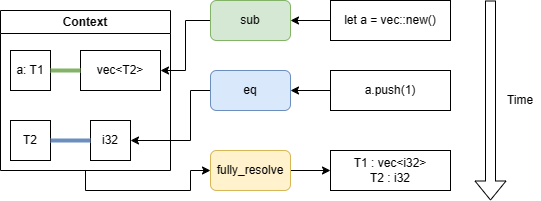
\includegraphics[width=120mm, height=45mm]{../img/RustTypeInference.png}
\caption{Rust type inference}
\label{img57:rustTypeInference}
\end{figure}
\par
\info{Properties of the type inference. More source of type info, Probing, Snapshots, No overloading}
The mentioned sharing of context enables type inference to be a back forward, meaning that based on future type information, it is possible to infer already collected unbounded type variables. 
Besides sharing the context, there are other inference features that are missing in C\# type inference and would be valuable. 
The first of them is type inference in object creation expressions, which doesn't exist in C\#. 
The next regards collecting type constraints, which are obtained from a wider context than C\# uses. 
For example, If a generic method containing a type variable in the return type is used as an assignment of an already typed variable, the type variable is constrained by the type of the target. Other features regard the inner implementation of type inference, which offers probing to constrain a type variable without influencing the context. 
There is a possibility of a snapshot that records all changes and can be used for backtracking and finding the right inferred type arguments.
Although Rust type inference is more advanced in comparison with C\#, we have to still consider language differences making type inference computation cost and difficulty relative to their features. As an example we can mention overloading causing already mentioned computation cost. 
Since Rust doesn't have overloading, the type inference can be more powerful without significant slowdown, which is not the case of C\#.

\section{Github issues}

\info{Intro}
The last subsection mentions the C\# developer's environment, where everybody is free to share his/her thoughts about possible improvements or issues with C\# language or Roslyn compiler.
We base our solution on issues mentioned in this section and recommended future possible features by C\# developers in the already mentioned the C\# language and Roslyn repository.
\par
\info{Proposal}
The process of designing a new language feature starts with publishing an idea into discussions \cite{online:discussions}, where the C\# community can comment on it. 
The idea contains a brief description of the feature, motivation, and design. 
Besides the idea, a new language feature requires a proposal, initially published as an issue, describing the feature in a way that can be later reviewed by the \ac{LDM} committee.
If the proposal sufficiently merits the discussions, it can be marked as a \textit{champion} by a member of \ac{LDM} for being discussed further by the team. 
There are several milestones in which the proposal can be. 
The most important for us is \textit{AnyTime}, meaning that the proposal is not actively worked on and is open to the community to collaborate on it. 
At the time of writing, a member of \ac{LDM} recommended championed issue \cite{online:champion} to be investigated since it contains many related discussions with proposed changes but still doesn’t have a required proposal. 
When a proposal has sufficient quality to be discussed by \ac{LDM}, a member invites the proposer to make a \textit{Pull Request} where further collaboration continues. 
If \ac{LDM} accepts the proposal, it is added to the \textit{proposals} folder in the repository for being added into the C\# specification, and its future implementation (in Roslyn) will be shipped with the next C\# version. 
\par
\info{Discussions}
Regarding the mentioned issue, we present related discussions directly or indirectly referred from it.
\par
\info{Discussion - Default type parameters}
The first discussion \cite{online:DefTypeParam} mentions \textit{Default type parameters} introducing default type arguments, which are used when explicit type arguments are not used. 
Figure \ref{img59:defTypeParam} shows a potential design of this feature where construing generic type \texttt{A} doesn’t need a type argument since it uses \texttt{int} type as a default value. 
\par
\begin{figure}
\begin{lstlisting}[style=csharp]
var temp = new A();

class A<T = int> {}
\end{lstlisting}
\caption{Default type parameters.}
\label{img59:defTypeParam}
\end{figure}
\par
\info{Discussion - Generic aliases}
The next discussion \cite{online:GenAlias} mentions \textit{Generic aliases} allowing to specify default values similar to the goal of the previous discussion by defining an alias to that type with option generic parameters. 
We can see an example of usage in Figure\ref{img60:genAlias}, where we predefine the first type argument of the \texttt{Dictionary} class to be the \texttt{string} type, which simplifies the usage of that type in scenarios where we often use dictionaries with keys of the \texttt{string} type.
\par
\begin{figure}
\begin{lstlisting}[style=csharp]
var temp = new StringDictionary<int>();

using StringDictionary<TValue> = Dictionary<String, TValue>;
\end{lstlisting}
\caption{Generic aliases.}
\label{img60:genAlias}
\end{figure}
\par
\info{Discussion - Named type arguments}
Discussion \cite{online:NamedTypeParam} mentions \textit{Named type parameters}, which are similar to named parameters of methods. 
The basic thought of this idea is being able to specify a type parameter for which we provide a type argument by name. 
In Figure \ref{img61:NamedTParam}, we can see a generic method \texttt{F} with two type parameters. 
With the current type inference, we have to always specify type arguments in method calls of \texttt{F}. 
We can tell the compiler specific type parameters for which we provide type arguments, \texttt{U} in this case,  using the named type arguments and letting the compiler infer the rest of the type parameters.
\par
\begin{figure}
\begin{lstlisting}[style=csharp]
var x = F<U:short>(1);

U F<T, U>(T t) { ... }
\end{lstlisting}
\caption{Named type parameters.}
\label{img61:NamedTParam}
\end{figure}
\par
\info{Discussion - Using char as inferred type argument}
Comments of the mentioned championed issue \cite{online:champion} propose several keywords that can be used in a type argument list for skipping type arguments, which can be inferred by the compiler and just providing the remaining ones. 
In example \ref{img62:CharITArg}, we can see the \texttt{var} keyword for skipping the first type argument since it can be inferred from the argument list, and we just specify the second type argument, which can’t be inferred by the compiler. 
The comments propose other options for keywords like underscore or whitespaces.
\par
\begin{figure}
\begin{lstlisting}[style=csharp]
Foo<var, int>("string");

TResult Foo<T, TResult>(T p1){ ... }
\end{lstlisting}
\caption{Using char as inferred type argument.}
\label{img62:CharITArg}
\end{figure}
\par
\info{Discussion - Inference based on target}
Discussion \cite{online:RetTInference} proposes \textit{Target-typed inference}, where type inference uses type information of the target assigned by the return value. 
We can see the usage in Figure \ref{img62:RetTInf}, where type inference determines that the return type has to be \texttt{int} type and uses that to deduce the type argument \texttt{T}.
\par
\begin{figure}
\begin{lstlisting}[style=csharp]
object row = ...
int id = row.Field("id")

static class ObjectEx {
	T Field<T>(this object target, string fieldName) 
	{ ... }
}
\end{lstlisting}
\caption{Target-typed inference.}
\label{img62:RetTInf}
\end{figure}
\par
\info{Discussion - Type inference based on type constraints}
The next idea of improving type inference is given by discussion \cite{online:TInfConst} , where type inference utilizes type information obtained from type constraints.
A simple example of that can be seen in Figure \ref{img63:TInfConst}, where \texttt{T1} can be deduced by using \texttt{T1}'s constraint and inferred type of \texttt{T2} forming inferred type \texttt{List<int>}.
\par
\begin{figure}
\begin{lstlisting}[style=csharp]
var temp = Foo(1);

T1 Foo<T1,T2>(T2 item) where T1 : List<T2> {}
\end{lstlisting}
\caption{Type inference based on type constraints.}
\label{img63:TInfConst}
\end{figure}
\par
\info{Discussion - Type inference of method return type}
Discussion \cite{online:TMRetInf} mentions type inference of method return type known from Kotlin language.
We can see the usage in the following Figure \ref{img64:TMRetInf}, where the return type of method \texttt{Add} is inferred to be \texttt{int} based on the type of the return expression.
\par
\begin{figure}
\begin{lstlisting}[style=csharp]
public static Add(int x, int y ) => x + y;
\end{lstlisting}
\caption{Type inference of method return type.}
\label{img64:TMRetInf}
\end{figure}
\par
\info{Discussion - Specifying type arguments in method calls (Realocation)}
Issue \cite{online:Realloc} proposes a way to compact type argument lists of identifiers containing inner identifiers with argument lists. 
We can see an idea demonstrated in example \ref{img65:Realloc}, where the argument list of \texttt{A<T1>} type and the \texttt{Foo<T2>} method are merged, and the type arguments are split by a semicolon.
\par
\begin{figure}
\begin{lstlisting}[style=csharp]
A.Foo<int;string>();

static class A<T1> {
    public static void Foo<T2>(){}
}
\end{lstlisting}
\caption{Specifying type arguments in method calls (Realocation).}
\label{img65:Realloc}
\end{figure}
\par
\info{Discussion - Constructor type inference}
The last discussion \cite{online:CtorTInf}, which we mention here, regards \textit{Constructor type inference} enabling type inference for object creation expressions. 
The type inference can be seen in Figure \ref{img66:CtorTInf}, where the \texttt{T} type parameter of the \texttt{C<T>} generic type can be deduced by using type information from its constructor.
\par
\begin{figure}
\begin{lstlisting}[style=csharp]
var temp = new C<_>(1); // T = int

class C<T> { public C(T p1) {}}
\end{lstlisting}
\caption{Constructor type inference.}
\label{img66:CtorTInf}
\end{figure}
